Fido was implemented in the C++ programming language with minimal use of the standard library.  This was to enable cross-platform functionality, lightweight and speedy performance, and the ability to run on microcontrollers if necessary.  Class structures were created for neurons and neural networks making extensive use of the ``std::vector'' sequence container, however to facilitate the goal of minimal standard library reliance a custom vector template class was created.  In order to test Fido both a simulation environment and a hardware implementation were constructed and written minimal driver suites for interaction with inputs and outputs. 

\subsection{Simulation}

An asynchronous simulator was created using C++ and the SFML graphics library in order to test Fido's performance.  Multiple inputs were modeled for simulation with outlets for control both by a human operator using sliders and by programmed handlers using a bridge class.  Sensors included a microphone, light sensor, infrared light sensor, inertial measurement unit, and three axes of radio receivers allowing measurement from a radio beacon.  Multiple tasks were trained using both operator input and autonomous ``taskmaster'' programs to regulate positive and negative feedback.


\begin{figure}
	\centering
	\fbox{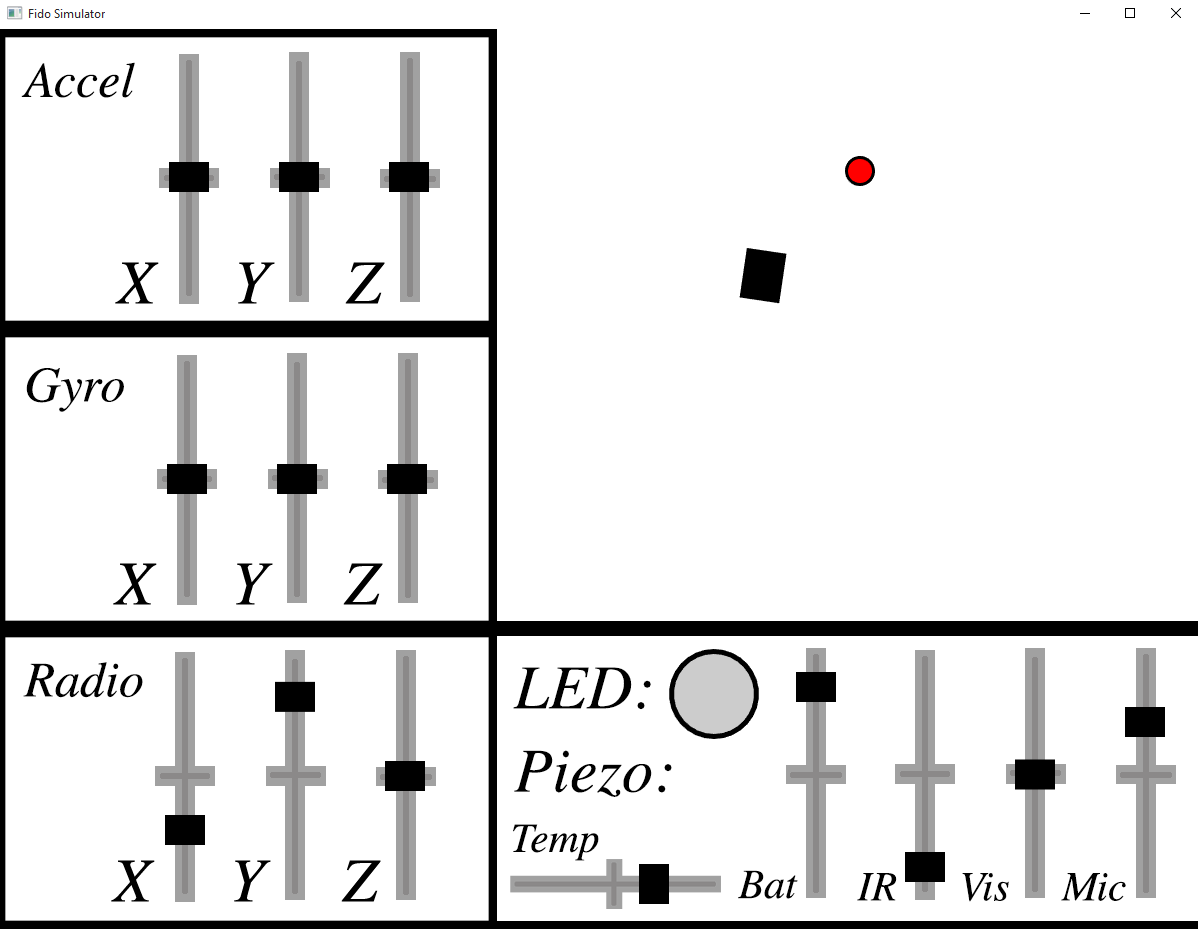
\includegraphics[height=10cm]{Figures/Screenshot.png}}
	\caption{Screenshot of the Fido Simulator Graphical User Interface}
\end{figure}

Fido's outputs were chosen similarly.  A buzzer of varying tone and frequency can play sounds and a multicolor LED can be lit to any red-green-blue color combination. Two motors allow movement using one of two kinematic configurations: differential drive similar to that of a tank, or holonomic control for each axis of movement.  Appropriate kinematics for each model including acceleration and friction were implemented with help from \cite{dudek}.

The black rectangle in the upper right corner of the simulator is the robot, having been moved as part of training.  The red dot near the rectangle is a graphical representation of a radio beacon.  As adjusting sliders to represent the location of a radio beacon relative to the robot would be impractical, we decided to implement a beacon that could be placed and dragged by right clicking on the simulator.  Simulated sensor readings of beacon strength on two axes are gathered using an inverse square law, as applies to radio waves in general.  These readings are then displayed in the sliders and can be manually altered as well.  The radio beacon can be removed by a human operator by pressing the ``p'' key in the simulator environment.  This was especially helpful in the task of training Fido to follow a radio beacon.
